
\chapter{Recolección de \textit{tweets} con RapidMiner}
\label{apendice:apendice1}

La recolección de \textit{tweets} para comprobar el dato teórico correspondiente a la existencia de menos de un 1\% de los \textit{tweets} de \textit{Twitter} contienen datos sobre su ubicación geográfica, se llevó a cabo haciendo uso de RapidMiner. Esta herramienta permite recolectar \textit{tweets} desde la API pública de \textit{Twitter} y generar estadísticas en base a ello.

Para su recolección se definió el proceso descrito en la Figura \ref{fig:RMP} corresponde a una iteración de $n$ veces sobre el subproceso descrito en la Figura \ref{fig:RMSP}, que es aquel que realiza la búsqueda de nuevos \textit{tweets}.

\begin{figure}[H]
        \centering
        \captionsetup{justification=centering}
        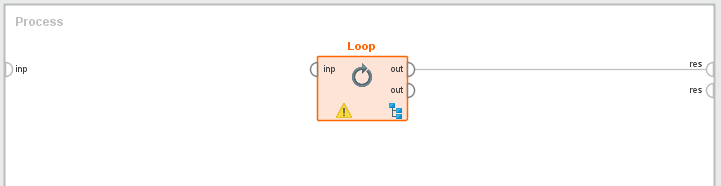
\includegraphics[scale=0.8]{images/RMProcess.png}
        \caption[Proceso de iteración en RapidMiner.]{Proceso de iteración en RapidMiner.\\Fuente: Elaboración Propia, (2016)}
        \label{fig:RMP}
\end{figure}

\begin{figure}[H]
        \centering
        \captionsetup{justification=centering}
        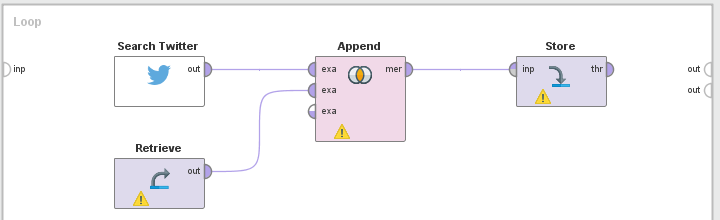
\includegraphics[scale=0.8]{images/RMSProcess.png}
        \caption[Subproceso de recolección de estados en RapidMiner.]{Subproceso de recolección de estados en RapidMiner.\\Fuente: Elaboración Propia, (2016)}
        \label{fig:RMSP}
\end{figure}

Se recolectaron 67.789 \textit{tweets} sólo con el idioma español en diferentes fechas, pues no se era capaz de obtener gran cantidad de datos debido a las limitaciones de \textit{Twitter}. Sin importar el resto de los campos sólo se centra la atención en los correspondientes a la geolocalización presentados en la Figura \ref{fig:RMResult}. La columna \textit{Missing} indica que ese campo se encuentra vacío.

\begin{figure}[H]
        \centering
        \captionsetup{justification=centering}
        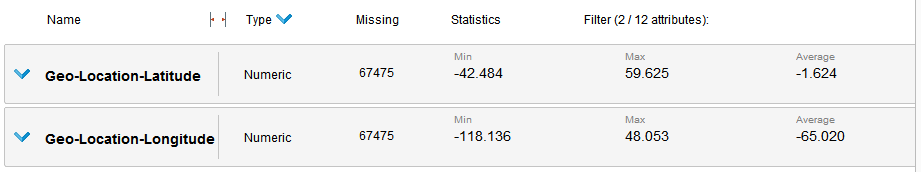
\includegraphics[scale=0.6]{images/ResultadoRapidMiner.png}
        \caption[Estadísticas de \textit{tweets} con geolocalización.]{Estadísticas de \textit{tweets} con geolocalización.\\Fuente: Elaboración Propia, (2016)}
        \label{fig:RMResult}
\end{figure}

Estos resultados señalan que sólo un 0.46\% de los datos allí muestreados cuentan con el campo de geolocalización con datos, lo que lleva a hacer creer que el valor descrito en la literatura es cierto y justifica aún más la necesidad del operador presentado en la sección \ref{subsec:detectorNecesidades}.

\chapter{Claves para el uso de la \textit{stream} API de \textit{Twitter}}
\label{apendice:clavesApi}

Para el uso de la API de \textit{Twitter} se requiere de cuatro \textit{tokens} de acceso. Estos pueden ser obtenidos por cualquier persona que posea una cuenta en la red social. Para obtenerlos se debe acceder a la página: \url{https://apps.twitter.com/}. Allí en la parte superior derecha se encuentra la opción \textit{"Create New App"} como se muestra en la Figura \ref{fig:CreateNewApp}.

\begin{figure}[H]
        \centering
        \captionsetup{justification=centering}
        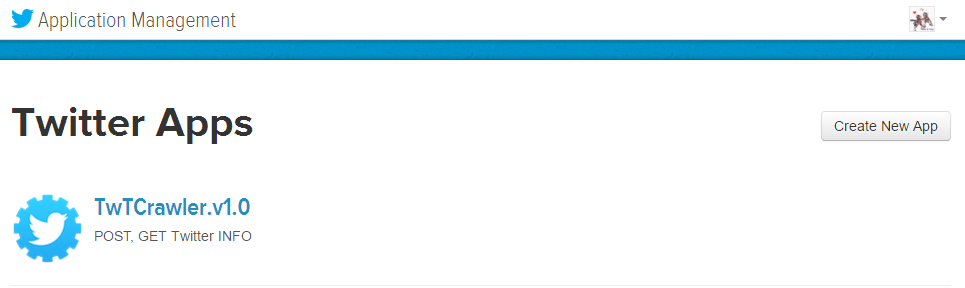
\includegraphics[scale=0.6]{images/CreateNewApp.png}
        \caption[Obtención de claves paso uno.]{Obtención de claves paso uno.\\Fuente: Elaboración Propia, (2016)}
        \label{fig:CreateNewApp}
\end{figure}

Una vez realizado lo anterior corresponde llenar los datos solicitados como se muestra en la Figura \ref{fig:CreateAnApp}, aceptar los términos de desarrollador expuestos al final de la página y presionar el botón \textit{"Create your Twitter application"}. 

\begin{figure}[H]
        \centering
        \captionsetup{justification=centering}
        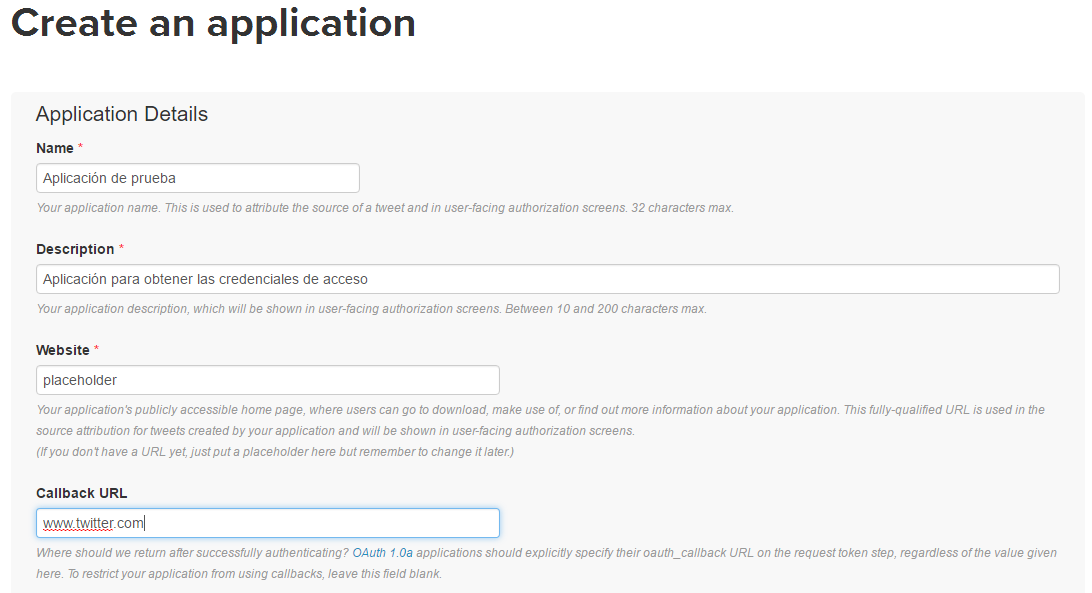
\includegraphics[scale=0.5]{images/CreateAnApplication.png}
        \caption[Obtención de claves paso dos.]{Obtención de claves paso dos.\\Fuente: Elaboración Propia, (2016)}
        \label{fig:CreateAnApp}
\end{figure}

La Figura \ref{fig:GetKey1} muestra el siguiente paso en la pestaña \textit{"Keys And Access Tokens"} donde se obtienen las primeras dos claves de acceso. La tercera y cuarta claves se obtienen presionando el botón \textit{"Regenerate Consumer Key and Secret"}, se solicitará confirmación y posterior a ello se redirige a la vista presentada en la Figura \ref{fig:GetKey1}. Para obtener las claves debe presionarse el botón \textit{"Test OAuth"}, se redirigirá a la página presentada en la Figura \ref{fig:TwitterKeys} donde se muestran todas las claves.

\begin{figure}[H]
        \centering
        \captionsetup{justification=centering}
        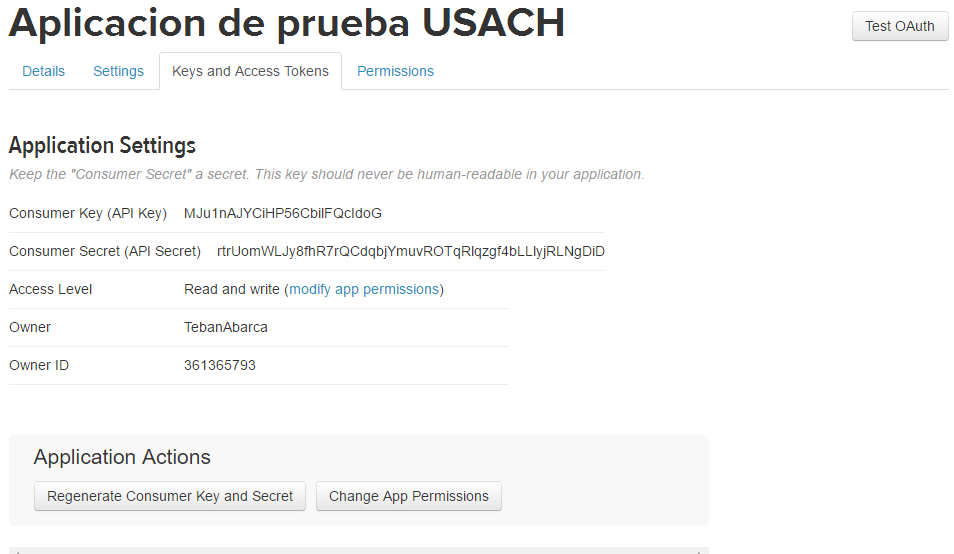
\includegraphics[scale=0.6]{images/GetToken1.png}
        \caption[Obtención de claves paso tres.]{Obtención de claves paso tres.\\Fuente: Elaboración Propia, (2016)}
        \label{fig:GetKey1}
\end{figure}

\begin{figure}[H]
        \centering
        \captionsetup{justification=centering}
        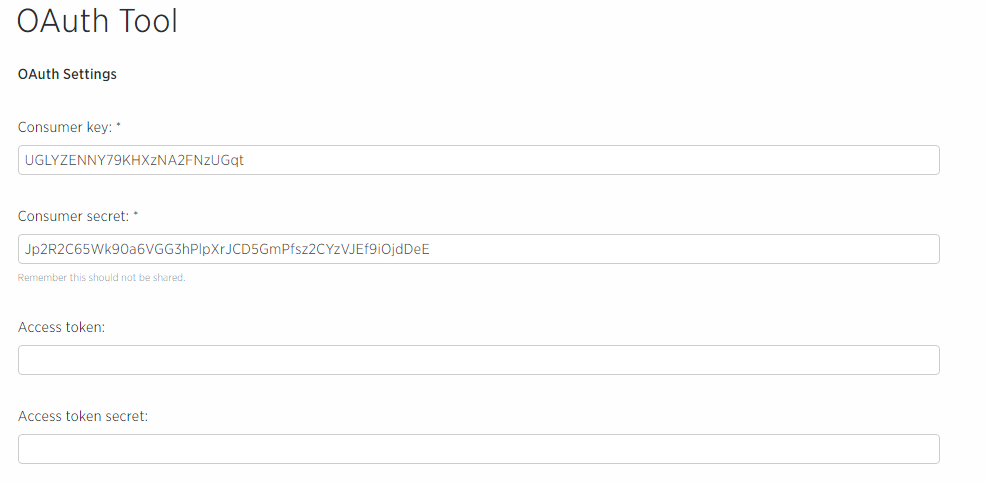
\includegraphics[scale=0.6]{images/TwitterKeys.png}
        \caption[Obtención de claves paso final.]{Obtención de claves paso final.\\Fuente: Elaboración Propia, (2016)}
        \label{fig:TwitterKeys}
\end{figure}

